\vfill
\pagebreak

\chapter{Computer science}

\section{Introduction}

\textbf{computer science} is an area of science that joins different theoretical disciplines (such as the creation of algorithms, computation theory, information theory, ...) and practical disciplines (hardware design, software implementation). We normally call “\textbf{computing}” the use, storage or processing of data and information in digital format.

A \textbf{computer system} is one that allows us to store and process data in digital format, to convert it into information. Normally a computer system is associated with computers (computers), which contain different components that we can use in our day to day.

\section{Brief history of computing/informatics}

The computers that we use today, and that we believe to be what we know as computing, is nothing more than an evolution of a set of ideas and advances that have occurred throughout history such as: logic, algebra, mechanics, electronics, creation of materials, ...

That is why we cannot think about the evolution of computing as something that has happened in recent decades, because it goes back several centuries. What follows is a small summary of a longer list that appears in the \href{https://es.wikipedia.org/wiki/Anexo:Historia_de_la_computaci%C3%B3n}{wikipedia}.

\begin{description}
    \item[1623] First mechanical calculator.

    \item[1666] The first calculator using wheels and gears is created.

    \item[1801] Through the use of punched cards, the mechanism of a weaving machine is controlled to make drawings and designs. (\href{https://www.youtube.com/watch?v=MQzpLLhN0fY}{Video})

    \item[1837] Charles Babbage describes the Analytical Engine. It is the design of a modern general purpose computer.

    \begin{minipage}{0.7\linewidth}
        \item[1843] \href{https://en.wikipedia.org/wiki/Ada_Lovelace}{Ada Augusta Lovelace} suggested the idea of punch cards being adapted in a way that would cause Babbage's engine to repeat certain operations. Because of this suggestion, some consider Lady Lovelace to be the \textbf{first programmer}.
    \end{minipage}
    \hfill
    \begin{minipage}{0.2\linewidth}
        \hfill
        \includesvg[width=\linewidth]{Ada_Lovelace_color.svg}
    \end{minipage}

    \item[1854] \href{https://en.wikipedia.org/wiki/George_Boole}{George Boole} publishes his \textbf{Boolean Algebra}. Because of the development of Boolean algebra, Boole is considered by many as the \textbf{father of computer theory}.

    \item [1912] \href {https://es.wikipedia.org/wiki/Leonardo_Torres_Quevedo}{Leonardo Torres Quevedo} builds an automaton capable of playing chess endings (rook and king against king) that he called “El ajedrecista”.

    \begin{center}
        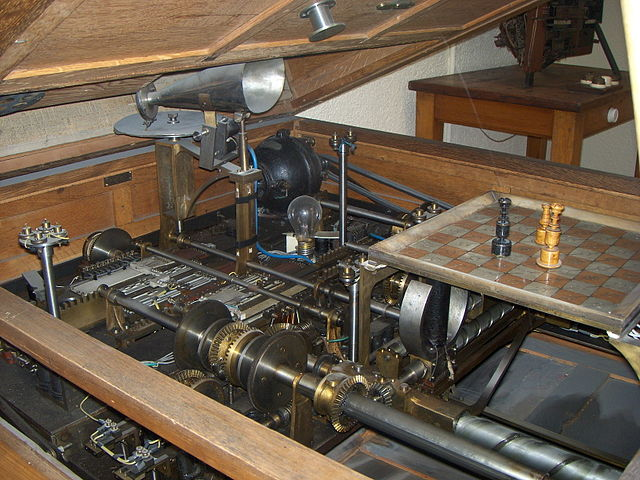
\includegraphics[width=0.7\linewidth]{ajedrecista.jpg}
        \captionof{figure}{El ajedrecista. Fuente: \href{https://es.wikipedia.org/wiki/El_Ajedrecista}{wikipedia}}
    \end{center}

    \item[1919]: American inventors W. H. Eccles and F. W. Jordan develop the first bistable or multivibrator circuit: the \textbf{flip-flop} in electronic lexicon. The flip-flop allowed the design of electronic circuits that could have two stable states, alternatively, thus being able to represent 0 as one state and the other as 1. This formed the basis for the storage and processing of the \textbf{binary bit}, a structure that current computers are used.

    \item [1924] Walther Bothe builds a logic gate \textbf {AND} for use in physical experiments, for which he received the Nobel Prize in Physics in 1954.

    \item[1936] Alan Turing describes the Turing machine, which formalizes the concept of an algorithm.

    \item[1938]: Konrad Zuse completes the first electromechanical computer, although not 100\% operational, the Z1.

    \item[1944] Colossus computers (Colossus Mark I and Colossus Mark 2) were built in England, with the aim of deciphering German communications during World War II.

    \item[1945] \href{https://es.wikipedia.org/wiki/John_von_Neumann}{John von Neumann} writes the “First Draft of a report on the EDVAC”, a page from the first document where the logical design of a computer is described using the concept of a stored-program. Today known as \textbf{von Neumann Architecture}.

    \item[1946] ENIAC (Electronic Numerical Integrator And Calculator) is built at the University of Pennsylvania, which was the first general purpose electronic computer

    \begin{center}
        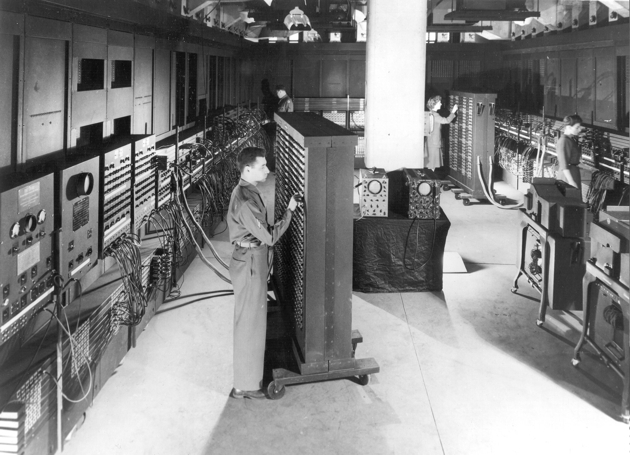
\includegraphics[width=0.7\linewidth]{ENIAC.jpg}
        \captionof{figure}{ENIAC. Source: \href{https://es.wikipedia.org/wiki/ENIAC}{wikipedia}}
    \end{center}

    \item[1951] The A-0 System was invented by \href{https://en.wikipedia.org/wiki/Grace_Murray_Hopper}{Grace Murray Hopper}. It was the \textbf{first compiler} developed for an electronic computer.

    \item[1958] The second generation of computers begins, characterized by using \textbf{transistorized circuits} instead of vacuum tubes.
\end{description}

Starting in the 1960s every year new systems were created that allowed what was already created to evolve.

\begin{description}
    \item[1964] The appearance of the IBM 360 marks the beginning of the third generation of computers. Integrated circuit boards begin.

    \item[1969] The first draft of what will be known as the ARPANET (the forerunner of today's Internet) is published.

    \item[1970] Intel creates the first dynamic RAM memory.

    \item[1971] Intel introduces the first commercial \textbf{processor} and at the same time the first microprocessor chip, the Intel 4004.

    \item[1971] Ray Tomlinson creates the first program to send email.

    \item[1972] Unix is rewritten, but using the C programming language.

    \item[1974] The Ethernet system is created to link through a single cable to the computers of a LAN.

    \item[1981] The \textbf{IBM PC} is released, becoming a commercial success, revolutionizing personal computing, and setting new standards.

    \item[1981] The \textbf{TCP/IP} protocol. We currently use it to browse the Internet.

    \vspace{10pt}
    \begin{minipage}{0.75\linewidth}
        \item[1983] \href{https://es.wikipedia.org/wiki/Richard_Stallman}{Richard Stallman} publicly announces the \href{https://es.wikipedia.org/wiki/GNU}{GNU} project, with the aim of create the first free Unix-like operating system.
    \end{minipage}
    \hfill
    \begin{minipage}{0.15\linewidth}
        \hfill
        \includesvg[width=\linewidth]{gnu.svg}
    \end{minipage}

    \item[1986] The \textbf{SQL} language is standardized by ANSI.

    \item[1990] \href{https://es.wikipedia.org/wiki/Tim_Berners-Lee}{Tim Berners-Lee} creates the \textbf{HyperText Markup Language} to create the World Wide Web (www), a new way of interacting with the Internet.

    \begin{minipage}{0.8\linewidth}
        \item[1991] Linus Torvalds begins developing Linux, the \textbf{kernel} of a Unix-compatible operating system.
    \end{minipage}
    \hfill
    \begin{minipage}{0.1\linewidth}
        \hfill
        \includesvg[width=\linewidth]{tux.svg}
    \end{minipage}

    \item[1991] Object-oriented programming begins to become popular.

    \item[1995] The first version of \href{https://es.wikipedia.org/wiki/MySQL}{MySQL} appears.

    \item[1995] The development of the server begins \href{https://es.wikipedia.org/wiki/Servidor_HTTP_Apache}{Apache}.

    \item[1997] The IEEE created the first WLAN standard and called it 802.11. The first protocol for WiFi.

\end{description}

More important moments could be added, but as previously said, only a small summary has been chosen.

\section{Components of a computer system}

A computer system has different components:

\begin{itemize}
    \item \textbf{Hardware}: Anything that is part of the computer, that \textbf{can be physically touched}: keyboard, mouse, monitor, motherboard, processor, memory, hard drive, cables, etc. It is the necessary “machinery” used for the automatic processing of information.

    \item \textbf{Software}: It is the logical element, it is everything that is “intangible”. It is the \textbf{set of programs and data} that allow the hardware to be managed, controlling and coordinating its operation so that it performs the desired tasks.

    Within the software we can differentiate (there are other possible categorizations):

    \begin{itemize}
        \item \textbf{System Software}: Programs that allow the administration of the hardware (the physical resources). They create a layer of abstraction between the hardware and the programs that the user uses. Within this section we can include: \textbf{operating systems}, \textbf{drivers} (controllers), diagnostic tools, ...

        \item \textbf{Development Software}: Programs that software developers use to create, debug, and maintain programs.

        \item \textbf{Application Software}: This category includes programs that have a specific function and are normally used by end users of the system.
    \end{itemize}

\end{itemize}
